%\documentclass[svgnames,table,mathserif,handout]{beamer}
\documentclass[svgnames,table,mathserif]{beamer}

\definecolor{red}{rgb}{1,0,0}

\newcommand{\notes}[1]{}

\mode<presentation>
{
  \usetheme{Warsaw}
  \setbeamercovered{transparent}
}
\useoutertheme{my}
\usecolortheme{dolphin}
\mode<handout>{\usecolortheme{dove}}
\usefonttheme{professionalfonts}

\usepackage{hyperref}
\usepackage[french]{babel}
\usepackage{times}
\usepackage[T1]{fontenc}
\usepackage[utf8]{inputenc}
\usepackage{epsfig}
\usepackage{graphicx}
\usepackage{psfrag}
\usepackage{amssymb}

\title{Proofs in Satisfiability Modulo Theories}

\author[]{C.~Barrett, L.~de Moura, P.~Fontaine}

\date{July 18, 2014}

\institute[]{%
}

\lecture{}{}

\AtBeginSection[]{%
  \begin{frame}%<beamer>
    \frametitle{Outline}
    \tableofcontents[currentsection]
  \end{frame}
}

\AtBeginSubsection[]{%
  \begin{frame}%<beamer>
    \frametitle{Outline}
    \tableofcontents[currentsection,currentsubsection]
  \end{frame}
}

\begin{document}

%--------------------------------------------------------------------- SLIDE --
%------------------------------------------------------------------------------

\begin{frame}

  \begin{center}

  {\huge Proofs in\\[8pt] Satisfiability Modulo Theories}\\

  \vspace*{20pt}
  Clark Barrett (NYU)\\[2pt]
  Leonardo de Moura (Microsoft Research)\\[2pt]
  Pascal Fontaine (Inria, Loria, U.\ Lorraine)

  \vspace*{10PT}\large
  APPA: All about Proofs, Proofs for All\\
  $\forall X\,.\,X\Pi$\\[5pt] July 18, 2014%\\[10pt]
%  \includegraphics[height=11mm]{LORIA.pdf}
  \end{center}
\end{frame}

\setbeamercovered{invisible}


%--------------------------------------------------------------------- SLIDE --
%------------------------------------------------------------------------------

\section{An overview of SMT solving}

\begin{frame}
  \frametitle{Satisfiability Modulo Theories $\approx$ SAT + expressiveness}

  \begin{block}{}
    \center
    Satisfiability of first-order formulas\\
    with interpreted and non-interpreted predicates and functions
  \end{block}

  {\footnotesize Interpreted: Axioms (e.g. arrays) or Structure (e.g. linear arithmetic)}

  \begin{itemize}
  \item SAT solvers\\
    \begin{center}
      $\neg \big[\left(p \Rightarrow q\right) \Rightarrow
      \big[\left(\neg p \Rightarrow q\right) \Rightarrow q\big] \big]$
    \end{center}
  \item congruence closure (uninterpreted symbols + equality)
    \begin{center}
    $a = b \wedge \big[ f(a) \neq f(b) \vee (p(a) \wedge \neg p(b))
    \big]$
    \end{center}
  \item in combination with arithmetic
    \begin{center}
    $a \leq b \wedge b \leq a + x \wedge x = 0 \wedge
      \big[ f(a) \neq f(b) \vee (p(a) \wedge \neg p(b + x)) \big]$
    \end{center}
  \item \dots
  \end{itemize}

  {\footnotesize
  E.g.: Alt-Ergo, Barcelogic, CVC4 (SVC, CVC, CVC-lite, CVC3),
  MathSAT, OpenSMT, SMTInterpol, veriT, Yices, z3 \dots}

\end{frame}

%--------------------------------------------------------------------- SLIDE --
%------------------------------------------------------------------------------

\begin{frame}[fragile]
  \frametitle{Standard input language: SMT-LIB 2.0}
  
  \begin{displaymath}
    a \leq b \wedge b \leq a + x \wedge x = 0 \wedge
    \big[ f(a) \neq f(b) \vee (q(a) \wedge \neg q(b + x)) \big]
  \end{displaymath}

\vspace*{5pt}
In SMT-LIB 2.0 format:
{\footnotesize
\begin{verbatim}
(set-logic QF_UFLRA)
(set-info :source | Example formula in SMT-LIB 2.0 |)
(set-info :smt-lib-version 2.0)
(declare-fun f (Real) Real)
(declare-fun q (Real) Bool)
(declare-fun a () Real)
(declare-fun b () Real)
(declare-fun x () Real)
(assert (and (<= a b) (<= b (+ a x)) (= x 0)
             (or (not (= (f a) (f b)))
                 (and (q a) (not (q (+ b x)))))))
(check-sat)
(exit)
\end{verbatim}
}

\end{frame}

%--------------------------------------------------------------------- SLIDE --
%------------------------------------------------------------------------------

\begin{frame}
  \frametitle{From propositional SAT to SMT}

  \begin{center}
\only<1>{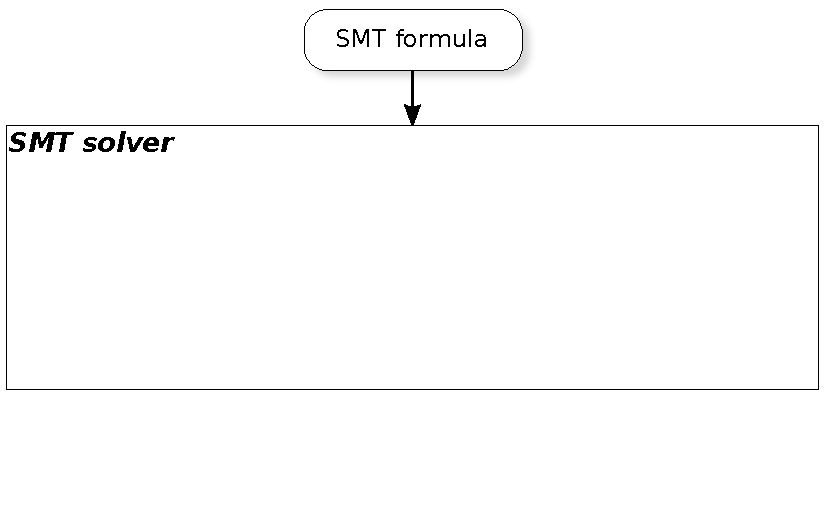
\includegraphics[height=0.5\textheight]{SMT1.pdf}}%
\only<2>{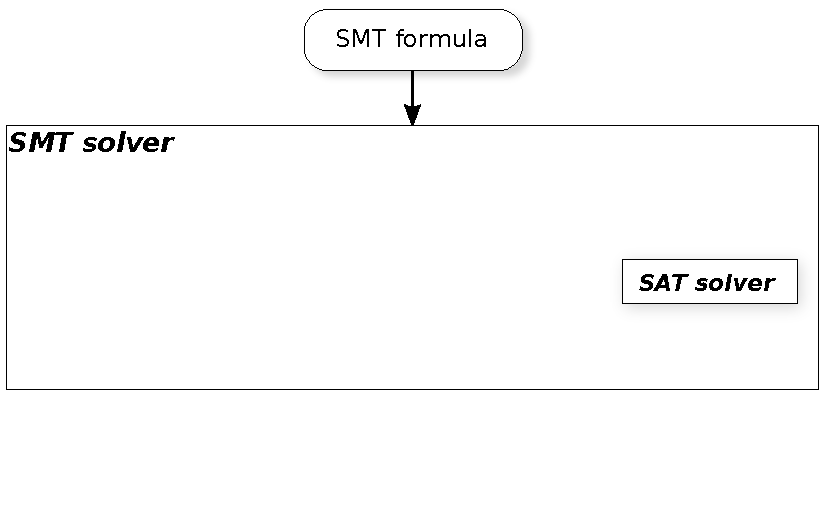
\includegraphics[height=0.5\textheight]{SMT2.pdf}}%
\only<3>{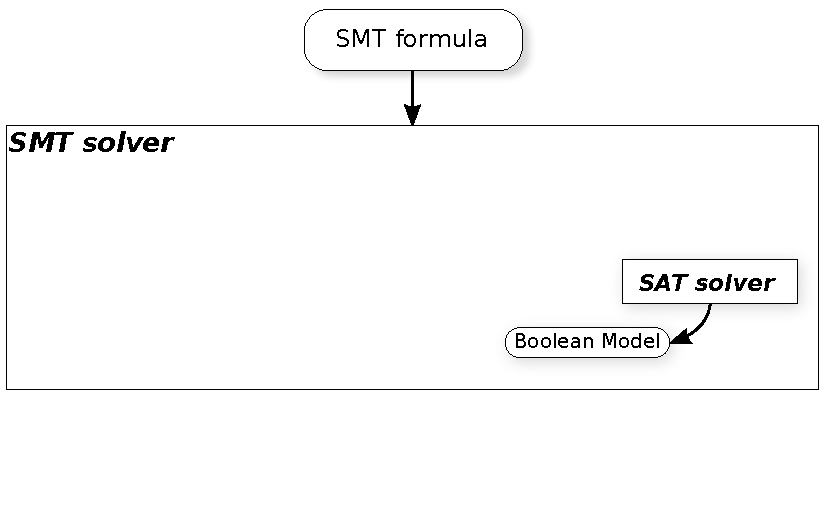
\includegraphics[height=0.5\textheight]{SMT3.pdf}}%
\only<4>{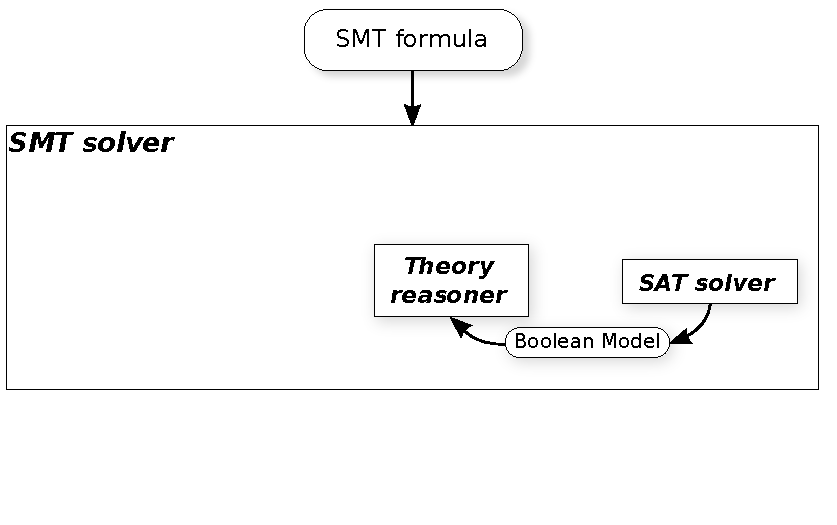
\includegraphics[height=0.5\textheight]{SMT4.pdf}}%
\only<5>{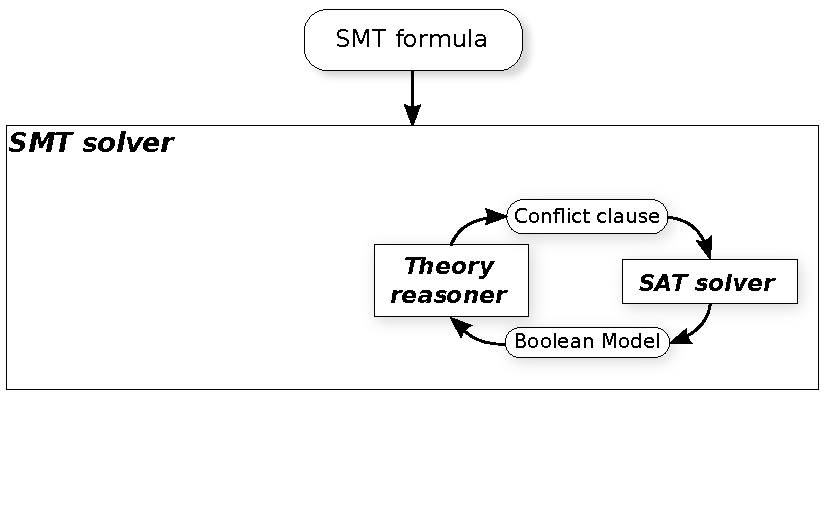
\includegraphics[height=0.5\textheight]{SMT5.pdf}}%
\only<6>{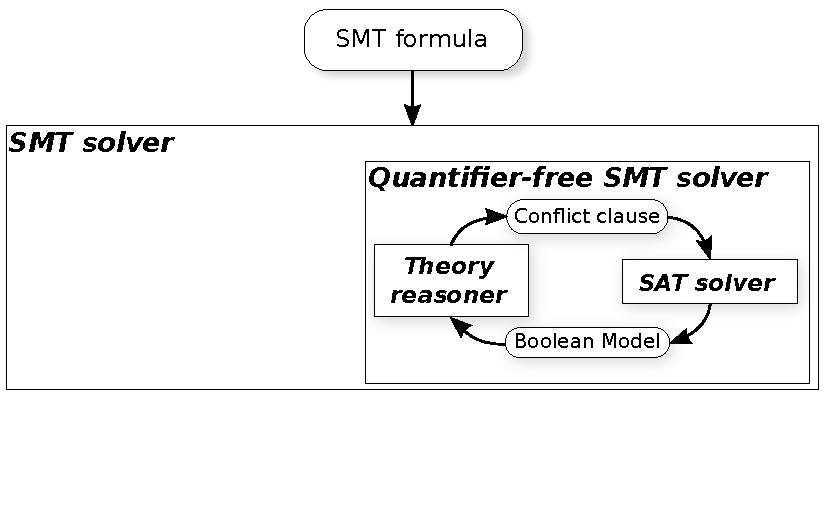
\includegraphics[height=0.5\textheight]{SMT6.pdf}}%
\only<7>{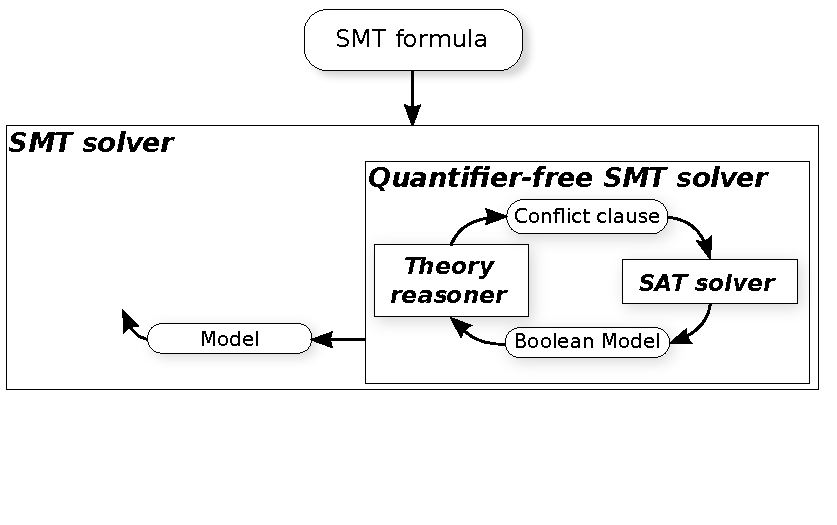
\includegraphics[height=0.5\textheight]{SMT7.pdf}}%
\only<8>{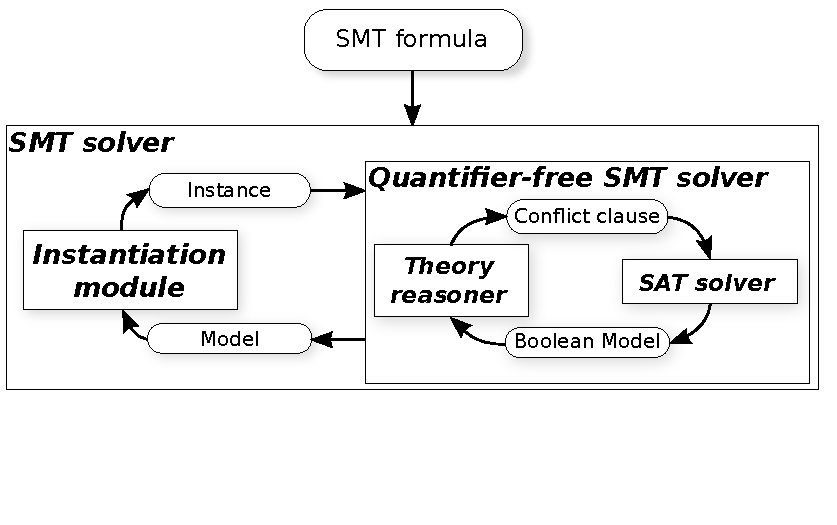
\includegraphics[height=0.5\textheight]{SMT8.pdf}}%
\only<9>{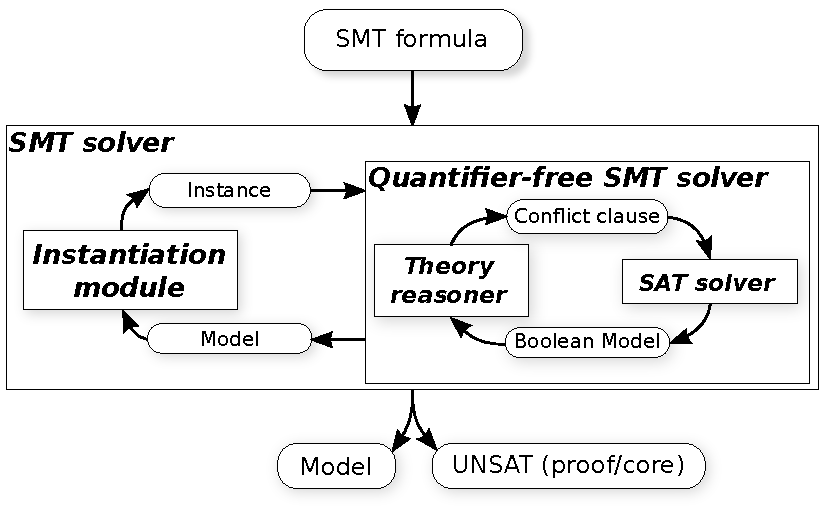
\includegraphics[height=0.5\textheight]{SMT9.pdf}}%
  \end{center}

\vspace*{-14pt}
\begin{footnotesize}
  Input: $a \leq b \wedge b \leq a + x \wedge x = 0 \wedge
  \big[ f(a) \neq f(b) \vee (q(a) \wedge \neg q(b + x)) \big]$

  \vspace*{2pt}
  \onslide<2->{
    To SAT solver: $p_{a \leq b} \wedge p_{b \leq a + x} \wedge p_{x = 0} \wedge
    \big[ \neg p_{f(a) = f(b)} \vee (p_{q(a)} \wedge \neg p_{q(b + x)}) \big]$}

  \vspace*{2pt}
  \onslide<3->{
    Boolean model: $p_{a \leq b}, p_{b \leq a + x}, p_{x = 0}, \neg p_{f(a) = f(b)}$}

  \vspace*{2pt}
  \onslide<4->{
    Theory reasoner: $a \leq b, b \leq a + x, x = 0, f(a) \neq f(b)$ unsatisfiable}

  \vspace*{2pt}
  \onslide<5->{New clause: $\neg p_{a \leq b} \vee \neg
    p_{b \leq a + x} \vee \neg p_{x = 0} \vee p_{f(a) = f(b)}$}

\end{footnotesize}

\end{frame}

%--------------------------------------------------------------------- SLIDE --
%------------------------------------------------------------------------------

\begin{frame}
  \frametitle{From propositional SAT to SMT: in practice}

  \begin{itemize}
  \item online decision procedures: theory checks propositional assignment on the fly
  \item small explanations: unsat core of propositional assignment\\
    discard classes of assignments (not one by one)
  \item theory propagation: instead of guessing propositional variable
    assignments, SAT solver assigns theory-entailed literals
  \item ackermannization, simplifications, and other magic
  \end{itemize}

\end{frame}

\section{Proofs and SMT}

  %% Theory and quantifier reasoning
  %% \begin{itemize}
  %% \end{itemize}



%% SMT proof: interleaving of SAT proof and theory reasoning proof

%% Challenge: collect enough information



%% Prooving Theory Lemmas

%% Congruence closure

%%  $a$, $b$, $f(a)$ and $f(b)$, the initial partition would be $\big\{\{a\},
%% \{b\}, \{f(a)\}, \{f(b)\}\big\}$

%% $\big\{\{a, b\}, \{f(a), f(b)\}\big\}$

%% $f(a) \neq f(b)$

%%  keeping a trace of which (two) terms are merged
%% and why (i.e.\ either because of a congruence, or an asserted equality).  This
%% information can be stored in an acyclic undirected\footnote{For efficiency
%%   reasons, modern congruence closure alogrithms actually use a directed
%%   graph~\cite{Nieuwenhuis6}.} graph




%% Linear Arithmetic

%% Farkas' lemma


%% Integers




%% Other theories
%% \begin{itemize}
%% \item arrays
%% \item inductive data types
%% \item bit-vectors
%% \item strings
%% \item non-linear arithmetic
%% \end{itemize}


%% Combination of theories

\section{Example of SMT proofs}

\begin{frame}[fragile]
\frametitle{CVC4 proof (1/3)}

{\tiny
\begin{verbatim}
(check
(% a var_real
(% b var_real
(% x var_real
(% f (term (arrow Real Real))
(% q (term (arrow Real Bool))
(% @F1 (th_holds (<=_Real (a_var_real a) (a_var_real b)))
(% @F2 (th_holds (<=_Real (a_var_real b) (+_Real (a_var_real a) (a_var_real x))))
(% @F3 (th_holds (= Real (a_var_real x) (a_real 0/1)))
(% @F4 (th_holds (or (not (= Real (apply _ _ f (a_var_real a)) (apply _ _ f (a_var_real b)))) 
                     (and (= Bool (apply _ _ q (a_var_real a)) btrue)
                          (= Bool (apply _ _ q (+_Real (a_var_real b) (a_var_real x))) bfalse))))
(: (holds cln)

(decl_atom (<=_Real (a_var_real a) (a_var_real b)) (\ v1 (\ a1
(decl_atom (<=_Real (a_var_real b) (+_Real (a_var_real a) (a_var_real x))) (\ v2 (\ a2
(decl_atom (= Real (a_var_real x) (a_real 0/1)) (\ v3 (\ a3
(decl_atom (= Real (a_var_real a) (a_var_real b)) (\ v4 (\ a4
(decl_atom (= Real (apply _ _ f (a_var_real a)) (apply _ _ f (a_var_real b))) (\ v5 (\ a5
(decl_atom (= Bool (apply _ _ q (a_var_real a)) btrue) (\ v6 (\ a6
(decl_atom (= Bool (apply _ _ q (+_Real (a_var_real b) (a_var_real x))) bfalse) (\ v7 (\ a7
(decl_atom (<=_Real (a_var_real b) (a_var_real a)) (\ v8 (\ a8
(decl_atom (= Real (a_var_real a) (+_Real (a_var_real b) (a_var_real x))) (\ v9 (\ a9
(decl_atom (and (= Bool (apply _ _ q (a_var_real a)) btrue)
                (= Bool (apply _ _ q (+_Real (a_var_real b) (a_var_real x))) bfalse))
  (\ v10 (\ a10
\end{verbatim}
}
\end{frame}

\begin{frame}[fragile]
\frametitle{CVC4 proof (2/3)}

{\tiny
\begin{verbatim}

; CNFication
(satlem _ _ (asf _ _ _ a1 (\ l1 (clausify_false (contra _ @F1 l1)))) (\ C1 
(satlem _ _ (asf _ _ _ a2 (\ l2 (clausify_false (contra _ @F2 l2)))) (\ C2 
(satlem _ _ (asf _ _ _ a3 (\ l3 (clausify_false (contra _ @F3 l3)))) (\ C3
(satlem _ _ (ast _ _ _ a5 (\ l5 (asf _ _ _ a6 (\ l6 (clausify_false (contra _
  (and_elim_1 _ _ (or_elim_1 _ _ (not_not_intro _ l5) @F4)) l6)))))) (\ C4
(satlem _ _ (ast _ _ _ a5 (\ l5 (asf _ _ _ a7 (\ l7 (clausify_false (contra _
  (and_elim_2 _ _ (or_elim_1 _ _ (not_not_intro _ l5) @F4)) l7)))))) (\ C5

; Theory lemmas
; ~a4 ^ a1 ^ a8 => false
(satlem _ _ (asf _ _ _ a4 (\ l4 (ast _ _ _ a1 (\ l1 (ast _ _ _ a8 (\ l8
 (clausify_false (contra _ l1
 (or_elim_1 _ _ (not_not_intro _ (<=_to_>=_Real _ _ l8)) (not_=_to_>=_=<_Real _ _ l4))))))))))
 (\ C6 
; a2 ^ a3 ^ ~a8 => false
(satlem _ _ (ast _ _ _ a2 (\ l2 (ast _ _ _ a3 (\ l3 (asf _ _ _ a8 (\ l8 (clausify_false
 (poly_norm_>= _ _ _ (<=_to_>=_Real _ _ l2) (pn_- _ _ _ _ _ (pn_+ _ _ _ _ _
  (pn_var a) (pn_var x)) (pn_var b)) (\ pn2
 (poly_norm_= _ _ _ (symm _ _ _ l3) (pn_- _ _ _ _ _ (pn_const 0/1) (pn_var x)) (\ pn3
 (poly_norm_> _ _ _ (not_<=_to_>_Real _ _ l8) (pn_- _ _ _ _ _ (pn_var b) (pn_var a)) (\ pn8
 (lra_contra_> _ (lra_add_>_>= _ _ _ pn8 (lra_add_=_>= _ _ _ pn3 pn2)))))))))))))))) (\ C7
; a4 ^ ~a5 => false
(satlem _ _ (ast _ _ _ a4 (\ l4 (asf _ _ _ a5 (\ l5 (clausify_false
 (contra _ (cong _ _ _ _ _ _ (refl _ f) l4) l5)))))) (\ C8
\end{verbatim}
}
\end{frame}

\begin{frame}[fragile]
\frametitle{CVC4 proof (3/3)}

{\tiny
\begin{verbatim}

; a3 ^ a4 ^ ~a9 => false
(satlem _ _ (ast _ _ _ a3 (\ l3 (ast _ _ _ a4 (\ l4 (asf _ _ _ a9 (\ l9 (clausify_false
 (poly_norm_= _ _ _ (symm _ _ _ l3) (pn_- _ _ _ _ _ (pn_const 0/1) (pn_var x)) (\ pn3
 (poly_norm_= _ _ _ l4 (pn_- _ _ _ _ _ (pn_var a) (pn_var b)) (\ pn4
 (poly_norm_distinct _ _ _ l9 (pn_- _ _ _ _ _ (pn_+ _ _ _ _ _
  (pn_var b) (pn_var x)) (pn_var a)) (\ pn9
 (lra_contra_distinct _ (lra_add_=_distinct _ _ _
  (lra_add_=_= _ _ _ pn3 pn4) pn9))))))))))))))) (\ C9
; a9 ^ a6 ^ a7 => false
(satlem _ _ (ast _ _ _ a9 (\ l9 (ast _ _ _ a6 (\ l6 (ast _ _ _ a7 (\ l7 (clausify_false
 (contra _ (trans _ _ _ _ (trans _ _ _ _ (symm _ _ _ l6) (cong _ _ _ _ _ _
  (refl _ q) l9)) l7) b_true_not_false)))))))) (\ C10

; Resolution proof
(satlem_simplify _ _ _ (R _ _ (Q _ _ (Q _ _ C6 C1 v1) (Q _ _ (Q _ _ C7 C2 v2) C3 v3) v8)
(Q _ _ (Q _ _ (Q _ _ (Q _ _ (R _ _ C9 C10 v9) C3 v3) C4 v6) C5 v7) C8 v5) v4)
(\ x x)))))))))))))))))))))))))))))))))))))))))))))))))))))))))))))))
\end{verbatim}
}

\end{frame}

\begin{frame}[fragile]
\frametitle{veriT proof (1/2)}

{\tiny
\begin{verbatim}
(set .c1 (input :conclusion ((and (<= a b) (<= b (+ a x)) (= x 0)
                               (or (not (= (f b) (f a))) (and (q a) (not (q (+ b x)))))))))
(set .c2 (and :clauses (.c1) :conclusion ((<= a b))))
(set .c3 (and :clauses (.c1) :conclusion ((<= b (+ a x)))))
(set .c4 (and :clauses (.c1) :conclusion ((= x 0))))
(set .c5 (and :clauses (.c1) :conclusion
           ((or (not (= (f b) (f a))) (and (q a) (not (q (+ b x))))))))
(set .c6 (and_pos :conclusion ((not (and (q a) (not (q (+ b x))))) (q a))))
(set .c7 (and_pos :conclusion ((not (and (q a) (not (q (+ b x))))) (not (q (+ b x))))))
(set .c8 (or :clauses (.c5) :conclusion
           ((not (= (f b) (f a))) (and (q a) (not (q (+ b x)))))))
(set .c9 (eq_congruent :conclusion ((not (= a b)) (= (f b) (f a)))))
(set .c10 (la_disequality :conclusion ((or (= a b) (not (<= a b)) (not (<= b a))))))
(set .c11 (or :clauses (.c10) :conclusion ((= a b) (not (<= a b)) (not (<= b a)))))
(set .c12 (resolution :clauses (.c11 .c2) :conclusion ((= a b) (not (<= b a)))))
(set .c13 (la_generic :conclusion ((not (<= b (+ a x))) (<= b a) (not (= x 0)))))
(set .c14 (resolution :clauses (.c13 .c3 .c4) :conclusion ((<= b a))))
(set .c15 (resolution :clauses (.c12 .c14) :conclusion ((= a b))))
(set .c16 (resolution :clauses (.c9 .c15) :conclusion ((= (f b) (f a)))))
(set .c17 (resolution :clauses (.c8 .c16) :conclusion ((and (q a) (not (q (+ b x)))))))
(set .c18 (resolution :clauses (.c6 .c17) :conclusion ((q a))))
(set .c19 (resolution :clauses (.c7 .c17) :conclusion ((not (q (+ b x))))))
\end{verbatim}
}

\end{frame}

\begin{frame}[fragile]
\frametitle{veriT proof (2/2)}

{\tiny
\begin{verbatim}
(set .c20 (eq_congruent_pred :conclusion ((not (= a (+ b x))) (not (q a)) (q (+ b x)))))
(set .c21 (resolution :clauses (.c20 .c18 .c19) :conclusion ((not (= a (+ b x))))))
(set .c22 (la_disequality :conclusion
            ((or (= a (+ b x)) (not (<= a (+ b x))) (not (<= (+ b x) a))))))
(set .c23 (or :clauses (.c22) :conclusion
            ((= a (+ b x)) (not (<= a (+ b x))) (not (<= (+ b x) a)))))
(set .c24 (resolution :clauses (.c23 .c21) :conclusion
            ((not (<= a (+ b x))) (not (<= (+ b x) a)))))
(set .c25 (eq_congruent_pred :conclusion
            ((not (= a b)) (not (= (+ a x) (+ b x))) (<= a (+ b x)) (not (<= b (+ a x))))))
(set .c26 (eq_congruent :conclusion ((not (= a b)) (not (= x x)) (= (+ a x) (+ b x)))))
(set .c27 (eq_reflexive :conclusion ((= x x))))
(set .c28 (resolution :clauses (.c26 .c27) :conclusion ((not (= a b)) (= (+ a x) (+ b x)))))
(set .c29 (resolution :clauses (.c25 .c28) :conclusion
            ((not (= a b)) (<= a (+ b x)) (not (<= b (+ a x))))))
(set .c30 (resolution :clauses (.c29 .c3 .c15) :conclusion ((<= a (+ b x)))))
(set .c31 (resolution :clauses (.c24 .c30) :conclusion ((not (<= (+ b x) a)))))
(set .c32 (la_generic :conclusion ((<= (+ b x) a) (not (= a b)) (not (= x 0)))))
(set .c33 (resolution :clauses (.c32 .c4 .c15 .c31) :conclusion ()))
\end{verbatim}
}

\end{frame}

\begin{frame}[fragile]
\frametitle{z3 proof (1/2)}

{\tiny
\begin{verbatim}
(let (($x82 (q b)) (?x49 (* (- 1.0) b)) (?x50 (+ a ?x49))
      ($x51 (<= ?x50 0.0)) (?x35 (f b)) (?x34 (f a))
      ($x36 (= ?x34 ?x35)) ($x37 (not $x36))
      ($x43 (or $x37 (and (q a) (not (q (+ b x))))))
      ($x33 (= x 0.0)) (?x57 (+ a ?x49 x)) ($x56 (>= ?x57 0.0))
      ($x44 (and (<= a b) (<= b (+ a x)) $x33 $x43))
      (@x60 (monotonicity (rewrite (= (<= a b) $x51))
                          (rewrite (= (<= b (+ a x)) $x56))
                          (= $x44 (and $x51 $x56 $x33 $x43))))
      (@x61 (mp (asserted $x44) @x60 (and $x51 $x56 $x33 $x43)))
      (@x62 (and-elim @x61 $x51)) ($x71 (>= ?x50 0.0)))
(let ((@x70 (trans (monotonicity (and-elim @x61 $x33) (= ?x57 (+ a ?x49 0.0)))
                   (rewrite (= (+ a ?x49 0.0) ?x50)) (= ?x57 ?x50))))
(let ((@x74 (mp (and-elim @x61 $x56) (monotonicity @x70 (= $x56 $x71)) $x71)))
(let ((@x121 (monotonicity (symm ((_ th-lemma arith eq-propagate 1 1) @x74 @x62 (= a b)) (= b a))
                           (= $x82 (q a)))))
(let (($x38 (q a)) ($x96 (or (not $x38) $x82)) ($x97 (not $x96)))
(let ((@x115 (monotonicity (symm ((_ th-lemma arith eq-propagate 1 1) @x74 @x62 (= a b)) (= b a))
                           (= ?x35 ?x34))))
(let (($x100 (or $x37 $x97)))
(let ((@x102 (monotonicity (rewrite (= (and $x38 (not $x82)) $x97))
                           (= (or $x37 (and $x38 (not $x82))) $x100))))
(let (($x85 (not $x82)))
(let (($x88 (and $x38 $x85)))
(let (($x91 (or $x37 $x88)))
(let ((@x81 (trans (monotonicity (and-elim @x61 $x33) (= (+ b x) (+ b 0.0)))
                   (rewrite (= (+ b 0.0) b)) (= (+ b x) b))))
(let ((@x87 (monotonicity (monotonicity @x81 (= (q (+ b x)) $x82)) (= (not (q (+ b x))) $x85))))
\end{verbatim}
}

\end{frame}

\begin{frame}[fragile]
\frametitle{z3 proof (2/2)}

{\tiny
\begin{verbatim}
(let ((@x93 (monotonicity (monotonicity @x87 (= (and $x38 (not (q (+ b x)))) $x88))
                          (= $x43 $x91))))
(let ((@x103 (mp (mp (and-elim @x61 $x43) @x93 $x91) @x102 $x100)))
(let ((@x119 (unit-resolution (def-axiom (or $x96 $x38))
                              (unit-resolution @x103 (symm @x115 $x36) $x97) $x38)))
(let ((@x118 (unit-resolution (def-axiom (or $x96 $x85))
                              (unit-resolution @x103 (symm @x115 $x36) $x97) $x85)))
(unit-resolution @x118 (mp @x119 (symm @x121 (= $x38 $x82)) $x82) false)))))))))))))))))
\end{verbatim}
}

\end{frame}

\section{Applications and Challenges}

\begin{frame}
  
  \begin{itemize}
    \item A standard for proofs
  \end{itemize}

\end{frame}



\end{document}

